% running.tex
%
% This is the `Running SCIRun' main section.

%begin{latexonly}
  \newcommand{\srwindow}%
  {\centerline{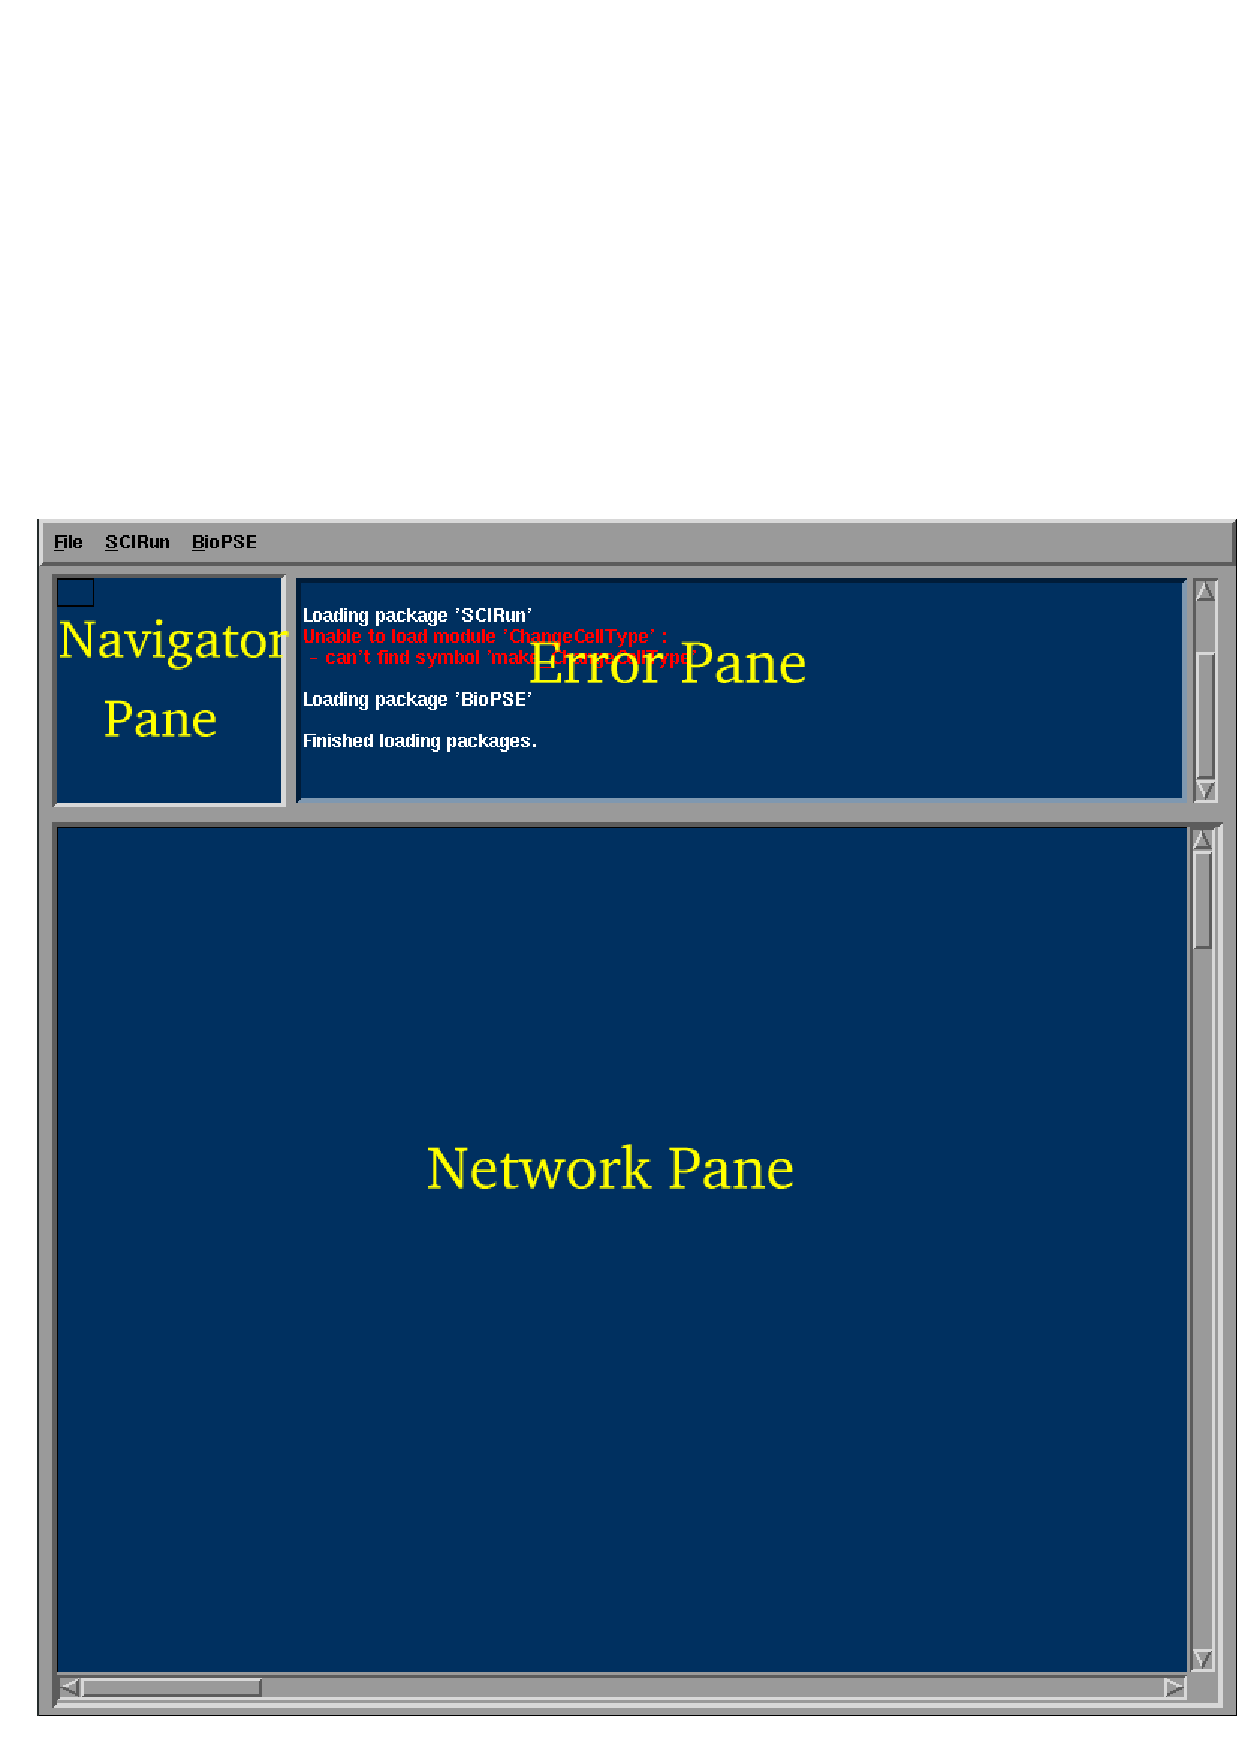
\epsfig{file=figures/srwindow-1.eps.gz,height=6in,
        bbllx=18, bblly=18, bburx=594, bbury=593}}}
%end{latexonly}
\begin{htmlonly}
  \newcommand{\srwindow}{%
  \htmladdimg[align=top,width=600,alt="SCIRun Window"]
  {../figures/srwindow-1.gif}}
\end{htmlonly}


\section{Starting \sr{}}
\label{sec:startingup}

\subsection{The \command{scirun} Command}
\label{sec:sciruncmd}

Start \sr{} by typing \keyboard{scirun} in a terminal (\eg \command{xterm})
window.  \note{Don't start \sr{} in the background, \ie don't type
\keyboard{scirun \&}}.

The \command{scirun} command is located in the
\directory{src} directory of the \directory{\sr} install directory.  The
person who installed \sr{} can locate this command for you.


\begin{figure}[htb]
  \begin{makeimage}
  \end{makeimage}
  \srwindow
  \caption{\label{fig:srwindow} \sr{} Main Window}
\end{figure}


Typing \keyboard{scirun} with no arguments starts up \sr{} with a blank \sr{}
window as shown in Figure~\ref{fig:srwindow}.  The main features of this
window are discussed in \secref{Anatomy of the Main
  Window}{sec:windowanatomy}.

The \command{scirun} command may take 1 argument
which is the name of a \sr{} \dfn{network} \index{network} file (these
files have a \filename{.net} extension).  These files hold previously
defined \sr{} networks.  \sr{} will load the specified network.  Network
files will be discussed in a later section.

\sr{} may encounter errors during start up.  These will be displayed in \sr{}'s
error message pane (see Figure~\ref{fig:srwindow}) (These errors should be
reported the \sr{} development team.  See \secref{Reporting Bugs}{sec:bugs} these
  errors.
this window shou

\subsubsection{Anatomy of the Main Window}
\label{sec:windowanatomy}

The \sr{} main window consists of 4 main components (see
Figure~\ref{fig:srwindow}): 

\begin{description}
\item[Menu Bar] The menu bar is used to load networks, save networks, quit
  \sr, create network modules, and perform other tasks.  The menu bar
  consists of the following menu items:

  \begin{description}
  \item[\menu{File}] The \menu{File} menu contains the following items:
    \begin{description}
    \item[Save] Saves the current network to a file.
    \item[Load] Loads a network from a file.
    \item[New] This submenu contains items of interest to developers only.
    \item[Add Info] Use this item to add network specific notes to
      the current network.  Notes should be used to document the purpose of
      the network.
    \item[Quit] Quits \sr.
    \end{description}
  \end{description}
  
  \begin{description}
  \item[\menu{SCIRun}] The \menu{SCIRun} menu is used to create modules
    (from the \sr{} package) for use in the network pane.  This menu is
    composed of submenus. Each submenu corresponds to a \dfn{category}
    \index{category} within the \sr{} package.  A category is group of
    related modules.  Each menu item in a category submenu creates a
    specific module and places it in the network pane.  The network pane's
    popup menu (activated by clicking the right most mouse button when the
    mouse pointer is in the network pane) also provides access to the
    \menu{\sr{}} and \menu{\pse{}} (and possibly other) package menus.  An
    overview of the contents of the \sr{} package is given in \secref{The
      \pse{} Package}{sec:biopsepackage}.
  \end{description}

  \begin{description}
  \item[\menu{BioPSE}] The \menu{BioPSE} menu is used to create modules
    (from the \pse package) for use in the network pane.  It consists
    of category submenus and module menu items.   An overview of the
    contents of the \sr{} package is given in \secref{The SCIRun
      Package}{sec:srpackage}.
  \end{description}

  \begin{description}
  \item [\textit{Other Package Menus}] There may be other package
    menus if other packages have been installed.  They too will consist
    of category submenus and module menu items.
  \end{description}
  
\item[Navigator Pane] The Navigator Pane is located in the upper left
  corner of the main window (see Figure~\ref{fig:srwindow}). It is used to
  navigate complex networks.  The use of the Navigator Pane will be
  described in \secref{Navigating a Network}{sec:navnetwork}.
  
\item[Error Pane] Errors during program startup are displayed in the Error
  Pane.  It is located in the upper right corner of the main window(see
  Figure~\ref{fig:srwindow}).  Errors on startup may mean that \sr{} has
  been installed incorrectly or has been installed from a buggy
  distribution.  Please \hyperref{report}{(see Section~}{)}{sec:bugs} these
  errors.
  
\item[Network Pane] The Network Pane occupies the bottom of the main
  window(see Figure~\ref{fig:srwindow}).  It is used to build and execute
  networks.  \secref{Building Networks}{sec:workwithnets} discusses the use
  of this pane.

\end{description}

\subsection{The Terminal Window}
\label{sec:termwinapp}

After starting, \sr{} will also run a shell-like application in the
terminal window called the \dfn{\sr{} shell}.  The \sr{} shell displays the
prompt \screen{scirun\ra}.  This program is actually a modified \dfna{Tool
  Command Language}{TCL} shell program and it is possible to type in
\acronym{TCL}'ish \sr{} commands at the prompt. The use of this program
will be described in \hyperref{a later section}{Section~}{}{sec:termapp}.


\subsection{\envvar{SCIRUN\_DATA}}
\label{sec:scirundata}

The environment variable \envvar{SCIRUN\_DATA} specifies the default
directory of \sr{} data files.  \sr will first look in this directory to
find data and network files.  It affects the behavior of file browsing
dialogs -- they will prompt for a file within the \envvar{SCIRUN\_DATA}
directory (of course you may have the dialog look elsewhere).


\subsection{Stopping}
\label{sec:stopping}

Quit \sr{} by selecting the \menuitem{Quit} item from the \menu{File} menu

\warning{Don't press \keyboard{control-c} to exit \sr.  Doing this will drop you into
a debugger which is probably not what you want to do}.


%%% Local Variables: 
%%% mode: latex
%%% TeX-master: "usersguide"
%%% End: 
